\subsection{Experimental Setup}
\paragraph{Procedure}
\begin{enumerate}
	\item 
	\item 
	\item 
\end{enumerate}
\paragraph{Variables}
\begin{enumerate}
    \item Voltage on function generator: 10V. (control)
	\item Probes 180º from each other. Sense leads 30º from the probe; 180º from each other(control)
	\item Gain $\frac{15k}{150} = 100$ (control)
	\item liquid volume 250 ml, 60mm height measured from inside the cup(control)
	\item Frequency (independent)
	\item Voltage peak-to-peak (dependent)
\end{enumerate}

\pagebreak 
\subsection{Raw data}
\begin{figure}[h]
\begin{minipage}{0.48\textwidth}
    \centering
    \begin{tikzpicture}[scale=0.85]
	    \begin{semilogxaxis}[
	    	title={PBS solution}, xlabel=Frequency $(\si{\hertz})$, ylabel=Amplitude $(\si{\milli\volt})$, ymin=10, ymax=30, %axis x line = bottom, axis y line=left,
	    ]
	    	\addplot[] table{PBS.dat};
	    \end{semilogxaxis}
    \end{tikzpicture}
    \caption{Amplitude based on frequency. Notice the dip at \SI{50}{\hertz} due to the filter.}
    \label{fig:}
\end{minipage}
\begin{minipage}{0.48\textwidth}
	\centering
	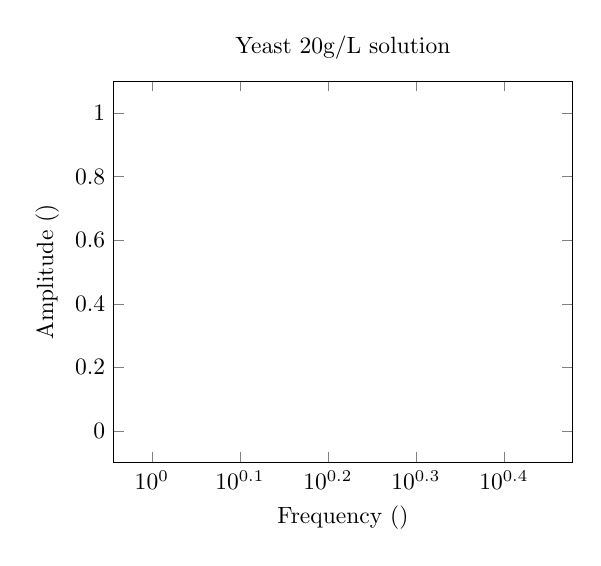
\begin{tikzpicture}[scale=0.85]
	\begin{semilogxaxis}[
	title={Yeast 20g/L solution}, xlabel=Frequency $(\si{\hertz})$, ylabel=Amplitude $(\si{\milli\volt})$
	]
%	\addplot[] table{};
	\end{semilogxaxis}
	\end{tikzpicture}
	\caption{}
	\label{}
\end{minipage}
\end{figure}


\begin{figure}[]
	\newcommand{\Radius}{3}
	\newcommand{\RadPow}{0.5}
	\newcommand{\RadVolt}{0.5}
	\centering
	\begin{tikzpicture}[legend entries = {Sensing electrodes, Driving electrodes}]
		\draw (0,0) circle (\Radius cm);
		%Driving electrodes
		\draw [dashed,cyan] (0,-\Radius) node{*} -- (0,\Radius) node{*};
		\node at (0.3,-\Radius-0.3) {-$V_x$};
		\node at (0.3,\Radius+0.3) {$V_x$}
		\draw [cyan]
			(0,\Radius) -- ++ (0,\RadPow)
			-- ++ ({-\Radius*1.3},0)
			-- ++ (0,{-\Radius-\RadPow)}) 
			++ (0,-\RadPow) circle (\RadPow) node{\mbox{\fontsize{25}{21.6}\selectfont\( \sim \)}} ++ (0,-\RadPow)
			-- ++ (0,{-\Radius+\RadPow})
			-- ++ ({\Radius*1.3},0)
			-- ++ (0,{\RadPow})
		; 
		% Sensor electrodes
		\draw[dashed, red] ({\Radius*cos(60)},{-\Radius*sin(60)}) node{*} -- ({-\Radius*cos(60)},{\Radius*sin(60)}) node{*} coordinate (a);
		\draw [red]
			(a) -- ++ (-{(2*\RadVolt*0.8)*cos(60)}, {(2*\RadVolt*0.8)*sin(60)}) coordinate (a)
			-- ++ (0,0) arc (-60:120:0.2)
			-- ++ ({1.3*\Radius*cos(30)},{1.3*\Radius*sin(30)})
			-- ++ ({(\Radius+\RadVolt)*cos(60)},{-(\Radius+\RadVolt)*sin(60)})
			++ ({\RadVolt*cos(60)},{-\RadVolt*sin(60)}) circle (\RadVolt) node{V} ++ ({\RadVolt*cos(60)},{-\RadVolt*sin(60)})
			-- ++ ({(\Radius+\RadVolt)*cos(60)},{-(\Radius+\RadVolt)*sin(60)})
			-- ++ ({-1.3*\Radius*cos(30)},-{1.3*\Radius*sin(30)})
			-- ++ ({(-2*\RadVolt*0.8)*cos(60)}, {(2*\RadVolt*0.8)*sin(60)})
		;
		%
		\draw [<->] (0,\Radius*0.5) arc (90:120:\Radius*0.5) node[pos=0.5,anchor=south]{$30º$};
	\end{tikzpicture}
	\caption{Orientation of electrodes}
	\label{fig:ElectrodeOrientation}
\end{figure}
\subsection{Analysis}
PBS numbers must be compared to yeast to tell us something meaningful regarding the frequency. At the moment, there is not much we can do.